\chapter{Tổng quan về mạng tương tác và bài toán phát hiện cộng đồng}\label{chap:c1}
\ifpdf
    \graphicspath{{Chapter1/Chapter1Figs/PNG/}{Chapter1/Chapter1Figs/PDF/}{Chapter1/Chapter1Figs/}}
\else
    \graphicspath{{Chapter1/Chapter1Figs/EPS/}{Chapter1/Chapter1Figs/}}
\fi
\section{Tổng quan về mạng tương tác}

Big Data là một thuật ngữ dùng để chỉ một tập hợp dữ liệu có kích thước lớn và phức tạp mà không thể xử lý trên những công cụ xử lý dữ liệu truyền thống. Thống kê cho thấy, trong hai năm qua khối dữ liệu trên toàn cầu đã chiếm đến $90\%$ lượng dữ liệu số được tạo ra kể từ khi công nghệ số hóa ra đời. Theo dự đoán của các chuyên gia dữ liệu nhận định rằng tốc độ tăng trưởng của dữ liệu là $62\%$ mỗi năm dự đoán đến năm $2020$ chúng ta sẽ có $40+$ exabytes. 

\begin{figure}[h]
	\centering
	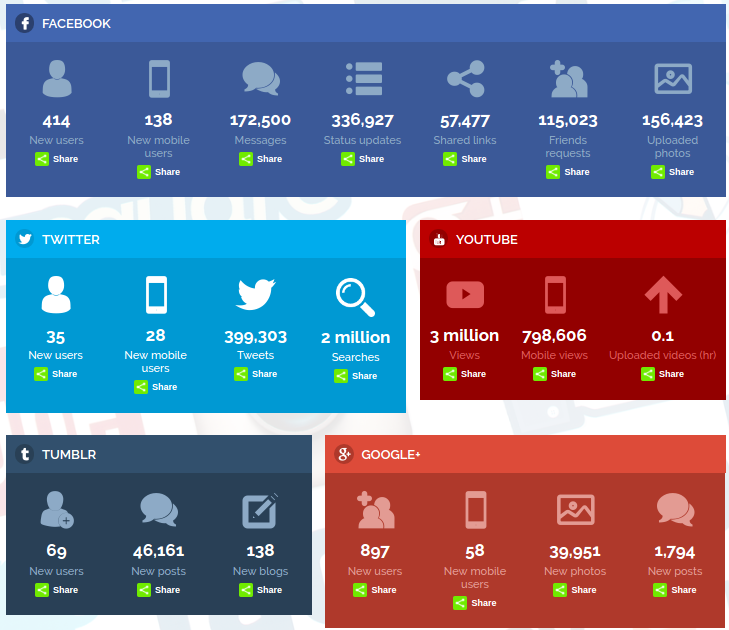
\includegraphics[width=0.6\linewidth]{Chapter1/Chapter1Figs/numberofsocialnetwork}
	\caption{Dữ liệu được sinh ra sau $60s$.}
	\label{fig:numbersocialnetwork}
\end{figure}

Nhìn vào hình \ref{fig:numbersocialnetwork} số liệu (2017)\footnote{http://www.coupofy.com/social-media-in-realtime} cho thấy trung bình cứ $60s$ mạng xã hội Facebook có $336,927$ status updates, $172,150$ mesages, $57,477$ shared links, $115,023$ friends requests,\dots Tương tự như Amazon, Google+, Youtube, Tweeter,\dots đều là những mạng tương tác vô cùng lớn là nơi lưu trữu các thông tin, quan điểm, tính cách, các tương tác giữa các cá thể,\dots Những thông tin này tạo thành đám mây tri thức vô cùng lớn mà chúng ta cần phải khai thác và đưa vào sử dụng. Có thể thấy trong kỷ nguyên số này thì dữ liệu chính là nguồn nhiên liệu vô cùng quan trọng của hầu hết các lĩnh vực. Việt Nam trong thời gian qua cũng đã và đang bắt đầu tiến đến cuộc cách mạng công nghiệp lần thứ tư thúc đẩy quá trình sản xuất thông minh dựa trên các thành tựu về công nghệ thông tin, công nghệ sinh học và công nghệ nano trong đó những bài toán về khai thác và xử lý dữ liệu được đặc biệt quan tâm. Theo lời của GS. Hồ Tú Bảo đã nói "Tới đây hầu hết các công ty đều phải sống dựa vào dữ liệu, ai có nhiều dữ liệu hơn và khai phá được nhiều hơn thì người đó sẽ thắng".

Nhìn nhận lại chúng ta thấy mạng tương tác xuất hiện trong nhiều lĩnh vực như: xã hội học, công nghệ thông tin, khoa học hành vi, toán học, thống kê, y học và nhiều lĩnh vực khác. Mạng tương tác hiện nay được chia ra thành các dạng khác nhau như mạng hiện - ẩn, tĩnh - động, ngoại tuyến - trực tuyến. Chủ yếu dữ liệu mạng tương tác được phân thành hai loại chính như sau:
\begin{itemize}
	\item Nội dung: Chính là các thông tin được lưu trữ trên mạng. Nội dung có thể được hiểu dưới nhiều góc độ khác nhau trong nhiều lĩnh vực như mạng xã hội là các thông tin, trạng khái, bình luận của người sử dụng hay trong mạng sinh học gen chính là các chỗi ADN thông tin. Do đó, kỹ thuật xử lý thường được sử dụng là các phường pháp xử lý văn bản. Tuy nhiên, do tính chất biến động và độ lớn của mạng xã hội hay tính không đầy đủ các thông tin được chia sẻ từ người dùng nên dữ liệu văn bản của mạng xã hội khác với các dữ liệu văn bản truyền thống trước đây. Những bài toán sử dụng dữ liệu này là: phân tích quan điểm người dùng trên mạng xã hội, tím kiếm chủ đề nổi bật trên mạng xã hội,\dots
	\item Cấu trúc: Chính là sự tương tác giữa các cá thể trong mạng. Ví dụ trong mạng xã hội là quan hệ kết bạn, like, share,\dots trong mạng thương mại là quan hệ mua hàng, bán hàng,\dots Cụ thể mạng tương tác được định nghĩa như là một mô hình đồ thị được cấu tạo bởi các đỉnh và các cạnh. Các đỉnh là tập các đối tượng, các cạnh là tập các tương tác giữa các cá thể. Các bài toán sử dụng dữ liệu này là: dự đoán liên kết trong mạng xã hội (được chia thành bốn bài toán con: dự đoán sự tồn tại của liên kết, dự đoán loại liên kết, dự đoán số liên kết, dự đoán số trọng số liên kết), gom nhóm hoặc phân lớp cộng đồng các các thể trong mạng (đây chính là bài toán sẽ được đề cập đến trong khóa luận này),\dots
\end{itemize}
\section{Bài toán phát hiện cộng đồng}
Theo định nghĩa của trên trang Oxford English Dictionary (2017)\footnote{https://en.oxforddictionaries.com/definition/community} thì từ "Communities: A group of people living in the same place or having a particular characteristic in common.". Có thể hiểu, cộng đồng là một nhóm các cá thể trong mạng có những tính chất tương tự nhau và cùng đóng một vai trò trong mạng. Chúng ta có ánh xạ khái niệm cộng đồng trong các mạng tương tác thường thấy như:
\begin{itemize}
	\item Mạng xã hội là một trong những ví dụ điển hình của đồ thị các cộng đồng. Con người có xu hướng kết nối với nhau lại với nhau, hình thành các nhóm (cộng đồng) trong cùng một môi trường làm việc, gia đình, bạn bè, sở thích,\dots
	\item Nghiên cứu y sinh học: Tương tác giữa các protein trong cùng một mô-đun (cộng đồng) sẽ có tính nổi trội hơn.
	\item Hệ khuyến nghị: Khách hàng có thể mua các sản phẩm từ nhóm các sản phẩm có liên quan đến nhau.
	\item \dots
\end{itemize}
 Như vậy nếu các protein, con người, hàng hóa là các tác nhân trong mạng thì các mô-đun, nhóm người dùng hay nhóm sản phẩm chính là các cộng đồng. Và nếu chúng ta phát hiện ra những cộng đồng tiềm năng này cho phép tạo ra nhưng giải pháp tốt nhất về chiến lượng kinh doanh, chữa ung thư, tăng năng suất bán hàng, điều tra tâm lý,\dots Hình\ref{fig:community1} là một ví dụ đơn giản của một mạng tương tác với ba cộng đồng. Dưới đây là phát biểu bài toán phát hiện cộng đồng trong toán học: 
 \nomenclature[KH]{$\mathcal{V}$}{Tập đỉnh}    
 \nomenclature[KH]{$\mathcal{E}$}{Tập cạnh}     
 \nomenclature[KH]{$G(\mathcal{V},\mathcal{E})$}{Đồ thị có $\mathcal{V}$ đỉnh và $\mathcal{E}$ cạnh}
  \nomenclature[KH]{$\mathcal{K}$}{Số cộng đồng}
  \nomenclature[KH]{$\mathcal{K}$}{Số cộng đồng}
  \nomenclature[KH]{$\mathcal{C}$}{Tập cộng đồng}    
 \begin{problem}(Phát hiện cộng đồng trong mạng)\label{def:ncdd1}
 	
 	Cho một đồ thị $G(\mathcal{V},\mathcal{E})$, chúng ta cần khám phá và phát hiện các cộng đồng $C_1,C_2,\dots,C_k$ với $\mathcal{K} \in {\mathcal{C}}$ là số lượng cộng đồng. Trong đó mỗi cộng đồng $C_i \subseteq \mathcal{V}$.
 \end{problem}
 
 Nếu ta thêm một ràng buộc trong bài toán là các $C_i$ là riêng biệt không có sự chồng chéo giữa chúng tức $C_i \cap C_j = \varnothing$, thì ta sẽ có một khái niệm mới cho bài toán \ref{def:ncdd1} là phát hiện cộng đồng không có sự chồng chéo (non-overlapping community detection). Ngược lại, bài toán khóa luận này đề cập đến chính là phát hiện cộng đồng ở đó $C_i$ có khả năng chồng chéo (overlapping community detection).
 
 Hay nói cách khác, phát hiện cộng đồng mạng hay có thể hiểu là việc phân cụm các đỉnh trong một mạng sử dụng cấu trúc mạng kết nối. Và $\mathcal{K}$ ở đây chính là số cộng đồng được ước lượng là tốt nhất.
 
 
\begin{figure}[h]
	\centering
	\begin{minipage}[b]{0.4\textwidth}
		\centering
		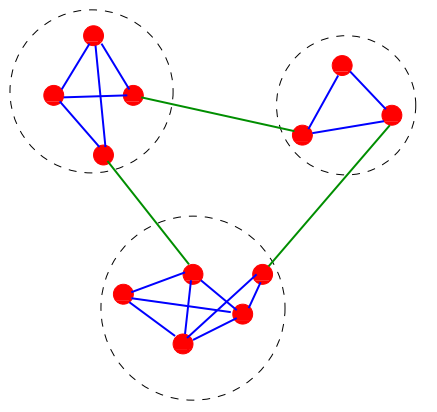
\includegraphics[width=1\linewidth]{Chapter1/Chapter1Figs/community-1}
		\caption{Một mạng tương tác (đồ thị) đơn giản với ba cộng đồng.}
		\label{fig:community1}
	\end{minipage}
	\begin{minipage}[b]{0.58\textwidth}
		\centering
		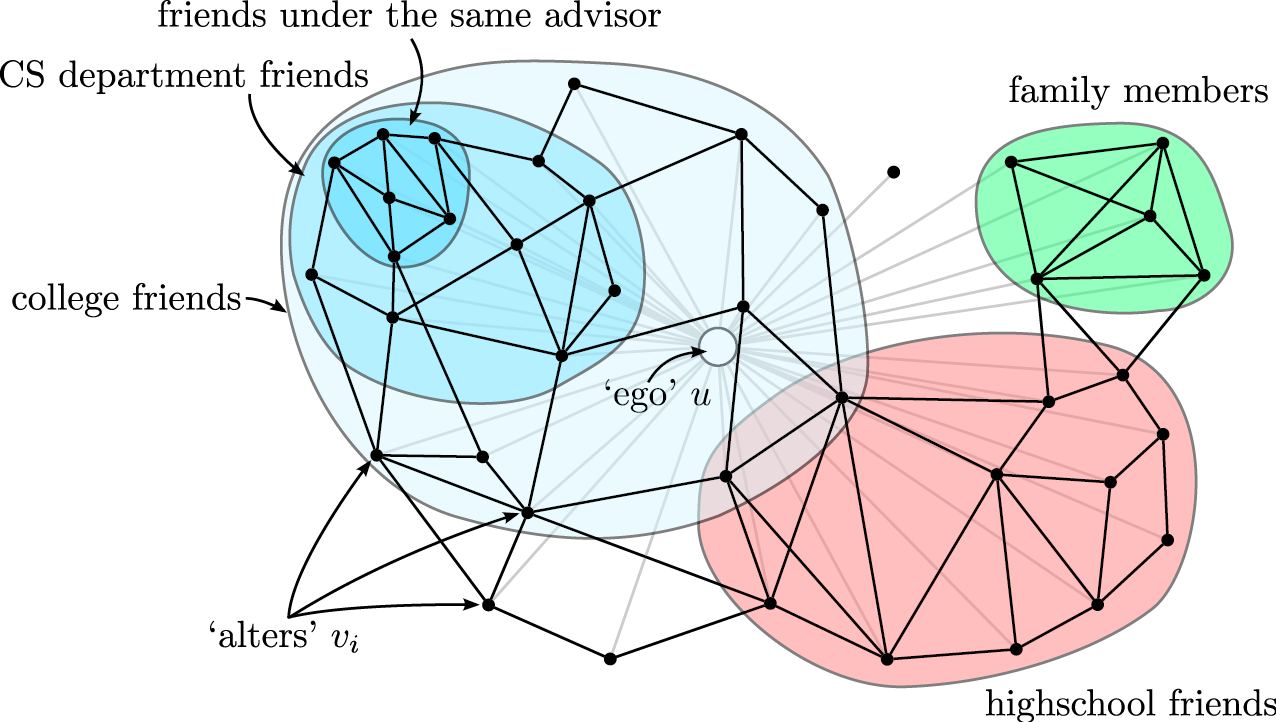
\includegraphics[width=1\linewidth]{Chapter1/Chapter1Figs/overlappingcommunity}
		\caption{Mô tả các cộng đồng trong mạng mạng cá nhân (egonetwork) của một sinh viên Đại học Stanford}
		\label{fig:overlapcommunity}
	\end{minipage}    
\end{figure}

Thực tế hầu như các cộng đồng giàu tính chồng chéo (giao nhau) hoặc là tập con của một cộng đồng khác. Có thể thấy rõ trong mạng xã hội, hình \ref{fig:overlapcommunity} là một kết quả của McAuley and
Leskovec [2012] \cite{DBLP2journals2corr2abs2121028182} cho thấy trong mạng cá nhân của sinh viên này có rất nhiều các cộng đồng khác nhau như family members, highschool fiends, college friends,\dots Và những cộng đồng này đều có tính chồng chéo và có cả những cộng đồng là con của một cộng đồng khác. Vì vậy bài toán phát hiện cộng đồng trong các mạng có đầy đủ cả ba loại cộng đồng như hình \ref{fig:typeofcommunity} là một bài toán khó trong khi sự bủng nổ về kích thước và độ phức tạp của các mạng tăng theo từng phút làm cho bài toán này càng trở lên khó khăn.

\begin{figure}[h]
	\centering
	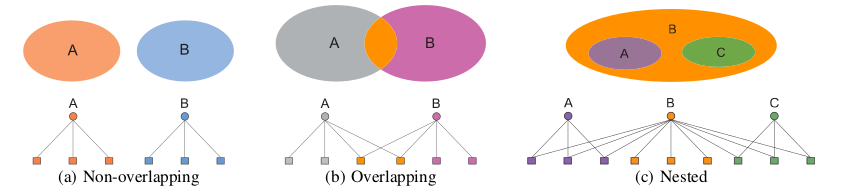
\includegraphics[width=\linewidth]{Chapter1/Chapter1Figs/typeofcommunity}
	\caption{Các loại cộng đồng mà trong mạng tương tác có thể có}
	\label{fig:typeofcommunity}
\end{figure}

Với tiềm năng đầy giá trị của bài toán cũng như những thách thức của bài toán đặt ra, chính là động lực để tôi chọn và thực hiện khóa luận này. Đề tài giải quyết bài toán phát hiện cộng đồng trong các mạng tương tác có kích thước lớn có tính không chồng chéo, chồng chéo và lồng (chứa) nhau trong thời gian cho phép. Trong các chương tiếp theo của khóa luận, tôi sẽ trình bày chi tiết giải quyết bài toán dựa trên mô hình BigCLAM được đề xuất bởi Yang and
Leskovec [2013] \cite{yang2013overlapping} kết hợp với một số phương pháp huấn luyện chạy trên hệ thống tính toán lưới.

\section{Một số nghiên cứu}
Bài toán phát hiện cộng đồng nhận được sự quan tâm từ rất sớm, và có rất nhiều phương pháp giải quyết bài toán \ref{def:ncdd1} có kết quả khá tốt. Tuy nhiên mỗi phương pháp đều có những khuyết điểm, thường khồng phù hợp các mạng có kích thước lớn hiện nay hoặc tỏ ra không vượt trội khi kích thước mạng tăng lên từng giây với thực tế.

\subsection{Phương pháp Girvan-Newman}
Phát hiện cộng đồng dựa trên việc tìm cạnh nối giữa các cộng đồng. Thuật toán này dựa trên quan niệm cho rằng khi các cộng đồng được gắn kết với nhau thì đường đi giữa các cộng đồng này đến cộng đồng khác sẽ đi qua các cạnh nối giữa chúng với tần suất cao. Điểm quan trọng nhất của phương pháp là xây dựng cộng đồng bằng cách loại bỏ dần dần các cạnh nói từ đồ thị ban đầu. Phương pháp này lần đầu tiên được đề xuất bởi Freeman. Theo Freeman, các cạnh được coi là cạnh có số lượng con đường ngắn nhất giữa các cặp đỉnh khác nhau chạy qua nó. Cạnh nối có ảnh hưởng rất lớn đến dòng chảy của thông tin giữa các nút khác, đặc biệt là trong trường hợp thông tin lưu truyền trong mạng chủ yếu theo con đường ngắn nhất. Phương pháp điển hình nhất trong sử dụng tính chất này là phương pháp Girvan-Newman của Newman [2004] \cite{newman2004fast}. Về cơ bản phương pháp Girvan-Newman được thực hiện theo các bước sau:
\begin{enumerate}
	\item Tính độ đo trung gian cho tất cả các cạnh trong mạng;
	\item Hủy bỏ các cạnh có độ trung gian cao nhất;
	\item Tính lại độ trung gian cho tất cả các cạnh bị ảnh hưởng theo các cạnh đã loại bỏ;
	\item Lặp tại từ bước 2 cho đến khi không con các cạnh trung gian ta sẽ có cộng đồng.
\end{enumerate}

\begin{figure}[H]
	\centering
	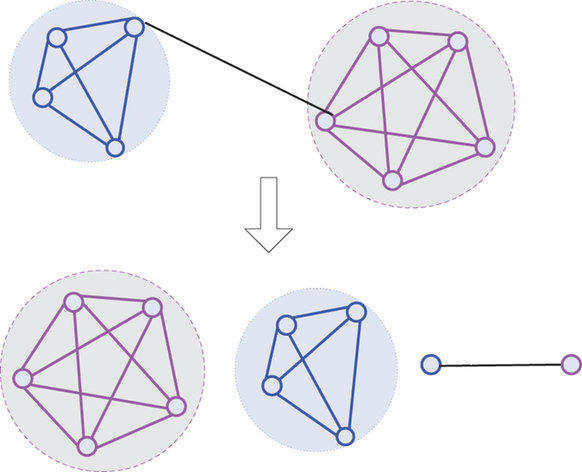
\includegraphics[width=0.5\linewidth]{Chapter1/Chapter1Figs/girvannewman}
	\caption{Minh họa phương pháp Girvan-Newman}
	\label{fig:girvannewman}
\end{figure}
Thuật toán Girvan-Newman khá đơn giản, dễ hiểu và có những kết quả tương đổi tốt trong nhiều trường hợp, mặc dù vậy nó vẫn gặp phải một số nhược điểm:
\begin{enumerate}
	\item Việc tính lại toàn bộ độ trung gian sau mỗi lần loại bỏ các cạnh có độ trung gian cao nhất. Như vậy khiến cho độ phức tạp của thuật toán rất lớn $O(m\times n)$ cho mỗi lần lặp với $m$ là số cạnh và $n$ là số đỉnh. Tổng thời gian chạy thuật toán là $O(m^n\times n)$, trường hợp xấu nhất, mỗi đỉnh là một cộng đồng thì độ phức tạp là $O(m^3)$. Như vậy dường như rất khó khả thi khi chạy trên mạng có kích thước lớn và phức tạp.
	\item Với phương pháp này thì toàn bộ cộng đồng thu được đều riêng biệt. Do vậy không thể làm việc hiệu quả trên mạng có các cộng đồng chồng chéo.
\end{enumerate}

\subsection{Phương pháp CONGA}
\nomenclature[KN]{CONGA}{Cluster Overlap Newman Girvan Algorithm}
Phương pháp CONGA viết tắt của từ Cluster Overlap Newman Girvan Algorithm là một phương pháp nâng cấp của phương pháp Girvan-Newman nhằm khắc phục nhược điểm không phát hiện được các cộng đồng chồng chéo nhau của thuật toán cũ. Các đỉnh sẽ được nhân bản hoặc gộp lại dựa vào một độ đo nhằm tính số cộng đồng mà đỉnh đó thuộc. Gregory [2007] \cite{gregory2007algorithm} đã đề xuất một độ đo đó được gọi là độ trung gian phân chia của đỉnh là số đường đi ngắn nhất mà chạy hai phần của đỉnh sau khi được phân chia. Như vậy với sự nâng cấp này phương pháp CONGA đã giải quyết được vấn đề chồng chéo cộng đồng, tuy nhiên vẫn tồn tại nhược điểm của phương pháp Girvan-Newman vẫn có độ phực tạp tính toán lớn.
\begin{figure}[H]
	\centering
	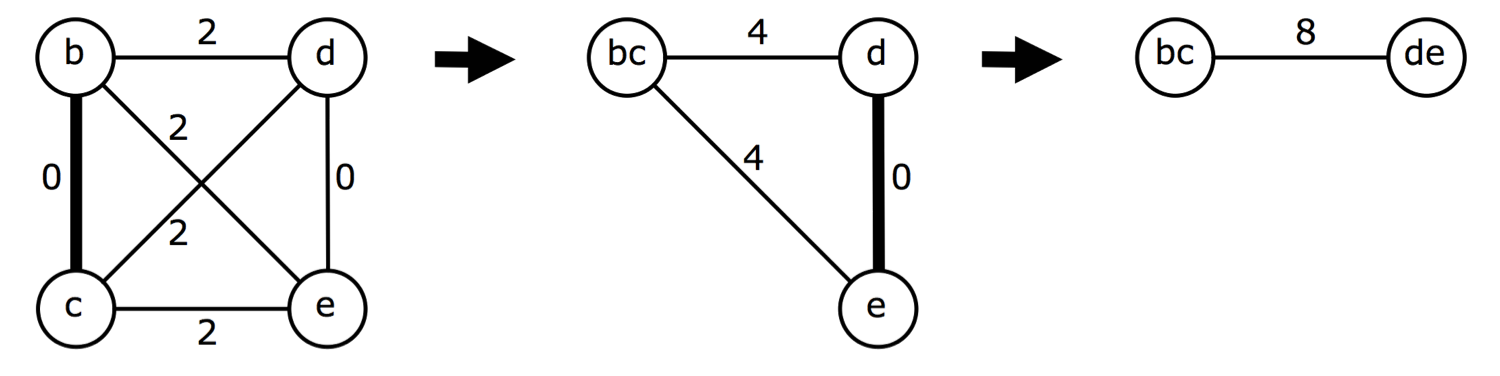
\includegraphics[width=0.8\linewidth]{Chapter1/Chapter1Figs/CONGA}
	\caption{Minh họa phương pháp CONGA}
	\label{fig:conga}
\end{figure}
\subsection{Affiliation Graph Model (AGM)}
\nomenclature[KN]{AGM}{Affiliation graph model}
\nomenclature[KH]{$M$}{Cạnh liên hết các đỉnh với các cộng đồng}
\nomenclature[KH]{$B(\mathcal{V},\mathcal{C},M)$}{Đồ thị hai phần thể hiện mô hình AGM}    
AGM được giới thiệu bởi Yang and Leskovec [2012] \cite{yang2012community} là mô hình xác suất xây dựng dựa trên một đồ thị hai phần (bigraph) $B(\mathcal{V},\mathcal{C},M)$ phần thứ nhất của đồ thị là các đỉnh $\mathcal{V}$ của mạng phần thứ 2 là các đỉnh định danh cho các cộng đồng trong mạng $\mathcal{C}$ mỗi cộng đồng sẽ được gắn với một xác suất $p_A$ kết nối giữa cộng đồng với các đỉnh được thể hiện qua cạnh nối $M$ giữa hai phần của đồ thị. AGM có khả năng phát hiện cộng đồng có tính chồng chéo không chồng chéo và lồng nhau trên mạng có kích thước lớn tương đối hiệu quả. Hình \ref{fig:agm} sẽ minh họa cho mô hình.

\nomenclature[KH]{$p_A$}{Xác suất của một cộng đồng} 

Mục tiêu của phương pháp phát hiện cộng đồng trên mô hình AGM là tìm  $\theta = B(\mathcal{V},\mathcal{C},M,\{p_c\})$:
\begin{equation}\label{ct:agm}
\arg \max_{B(\mathcal{V},\mathcal{C},M,\{p_c\})}{ \prod_{(u,v)\in \mathcal{E}}{p(u,v)}\prod_{(u,v)\notin \mathcal{E}}{(1-p(u,v))}}
\end{equation}
\begin{figure}[H]
	\centering
	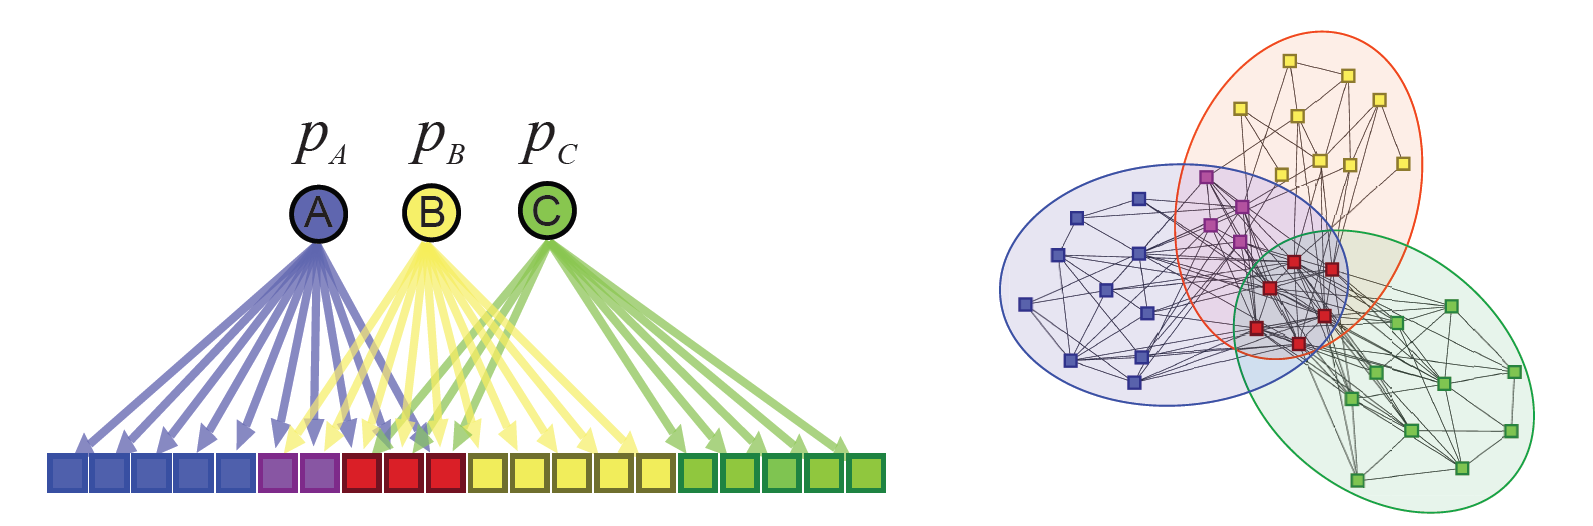
\includegraphics[width=0.8\linewidth]{Chapter1/Chapter1Figs/agm_g}
	\caption{Minh họa mô hình AGM}
	\label{fig:agm}
\end{figure}
Tuy nhiên, theo tác giả để tìm tìm được $B(\mathcal{V},\mathcal{C},M,\{p_c\})$ theo công thức \ref{ct:agm} không hệ đơn giản.

\subsection{Non-negative Matrix Factorization}
\nomenclature[KN]{NMF}{Non-negative Matrix Factorization} 
Non-negative Matrix Factorization (NMF) hay còn gọi phân tích tích matrix không âm thành nhân tử là một kỹ thuật được sử dụng phổ biến giải quyết các bài toán học máy (machine learning), học nhiều tầng (deep learning), hệ khuyến nghị (recommendation system),\dots Trong bài toán phát hiện cộng đồng, NMF tỏ ra khá vượt trội so với các phương pháp khác.

Trong khóa luận này, có đề cập đến mô hình BigCLAM của Yang and Leskovec [2013] \cite{yang2013overlapping} một sự nâng cấp từ mô hình AGM xây dựng dựa trên phương pháp NMF không chỉ trong bài phát hiện cộng đồng chồng chéo mà còn phát hiện được các cộng đồng không chồng chéo và cộng đồng lồng nhau với kết quả vượt trội hơn rất nhiều so với AGM. Mô hình BigCLAM xây dựng một đồ thị hai phần (bipartite graph) giống như AGM phần thứ nhất của đồ thị là các nốt định danh cho các cộng đồng trong mạng phần còn lại là các đỉnh của mạng và cạnh nối giữa các các hai phần của đồ thị chính là độ đo liên kết của các đỉnh trong mạng với các cộng đồng được biểu diễn thành vector. Chi tiết mô hình sẽ được trình bày chi tiết trong chương \ref{chap:c3}.